%%%%%%%%%%%%%%%%%%%%%%%%%%%%%%%%%%%%%%%%%
% MLE Release Meeting Deck
% Built from docs/presentation/template.tex
%%%%%%%%%%%%%%%%%%%%%%%%%%%%%%%%%%%%%%%%%

\documentclass[11pt,aspectratio=169]{beamer}

\graphicspath{{Images/}{Images/final/}}

\usepackage{amsmath}
\usepackage{amssymb}
\usepackage{booktabs}
\usepackage{palatino}
\usepackage[default]{opensans}

\usetheme{Madrid}
\useinnertheme{circles}
\setbeamertemplate{navigation symbols}{}
\setbeamertemplate{footline}[frame number]

\definecolor{DeepBlue}{HTML}{1F4E79}
\definecolor{SoftGray}{HTML}{F4F6F8}
\definecolor{CaveatRed}{HTML}{C62828}
\definecolor{CleanGreen}{HTML}{2E7D32}
\definecolor{WarmGold}{HTML}{F9A825}

\setbeamercolor{structure}{fg=DeepBlue}
\setbeamercolor{frametitle}{fg=white,bg=DeepBlue}
\setbeamercolor{title}{fg=DeepBlue}
\setbeamercolor{block title}{fg=white,bg=DeepBlue}
\setbeamercolor{block body}{bg=SoftGray,fg=black}
\setbeamercolor{alerted text}{fg=CaveatRed}

\newcommand{\claim}[1]{\begin{block}{}\large #1\end{block}}
\newcommand{\figsource}[1]{{\scriptsize\color{gray}Source: #1}}

\title[MLE-only posterior analysis]{What does releasing only \texorpdfstring{$\hat{\mu}$}{mu-hat} preserve, distort, and reveal?}
\subtitle{Correctness, efficiency, geometry, and privacy payoff from \texttt{final\_production\_v1}}
\author[Shlok Mishra]{Shlok Mishra}
\institute[CEREMADE]{CEREMADE Lab}
\date[June 2026]{Meeting discussion deck \\ June 2026}

\begin{document}

\begin{frame}
  \titlepage
\end{frame}

\begin{frame}{Talk map}
  \begin{enumerate}
    \item Build a reliable posterior reference for $p(\mu \mid \hat{\mu})$.
    \item Validate Gibbs and RATTLE against summaries and diagnostics.
    \item Compare cost per reliable posterior information.
    \item Use geometry to explain wins, failures, and caveats.
    \item Ask the statistical/privacy question: what does $\hat{\mu}$ leak?
  \end{enumerate}
\end{frame}

\section{Problem and Setup}

\begin{frame}{The problem}
  \claim{A released MLE is a compressed statistic. We want to understand the Bayesian posterior and the latent datasets still compatible with that release.}
  \[
    p(\mu \mid x_{1:n}) \quad \text{versus} \quad p(\mu \mid \hat{\mu}=\mu^\star)
  \]
  \begin{itemize}
    \item If the statistic is sufficient, little is lost.
    \item If not, the release may distort posterior uncertainty.
    \item The same release can also change beliefs about hidden latent extremes.
  \end{itemize}
\end{frame}

\begin{frame}{Models and regimes}
  \begin{columns}[T,onlytextwidth]
    \begin{column}{0.48\textwidth}
      \begin{block}{Main comparison regimes}
        \begin{itemize}
          \item Logistic: $n=10,20,50$
          \item Student: $k=2,3$, selected $n$
          \item Laplace: odd $n=11,21,51$, Gibbs only
        \end{itemize}
      \end{block}
    \end{column}
    \begin{column}{0.48\textwidth}
      \begin{block}{Caveat regimes}
        \begin{itemize}
          \item Student $k=1,n=10$: unresolved
          \item Student $k=1$: heavy-tail stress test
          \item Laplace RATTLE: not applicable
        \end{itemize}
      \end{block}
    \end{column}
  \end{columns}
\end{frame}

\begin{frame}{Frozen evidence source}
  \claim{\texttt{final\_production\_v1} is the meeting dataset.}
  \begin{columns}[T,onlytextwidth]
    \begin{column}{0.55\textwidth}
      \begin{itemize}
        \item 81 completed sampler case directories
        \item 100k iterations, 20k burn-in
        \item 3 seeds per production case
        \item 129,681 thinned latent geometry states
        \item 540 paired release-information datasets
      \end{itemize}
    \end{column}
    \begin{column}{0.38\textwidth}
      \begin{block}{Dashboard default}
        \texttt{results/dashboard\_cache/}\\
        \texttt{final\_production\_v1}
        \medskip

        Posterior page starts on Student $k=3,n=20$.
      \end{block}
    \end{column}
  \end{columns}
\end{frame}

\section{Reference Construction}

\begin{frame}{Reference hierarchy}
  \claim{Raw weighted-MC is the posterior-summary benchmark. KDE is a diagnostic smoothing layer for density displays.}
  \begin{columns}[T,onlytextwidth]
    \begin{column}{0.48\textwidth}
      \begin{block}{Raw weighted-MC}
        Direct weighted Monte Carlo summaries from $B=100{,}000$ weighted draws; no smoothing is applied before computing means, SDs, quantiles, and tail probabilities.
      \end{block}
    \end{column}
    \begin{column}{0.48\textwidth}
      \begin{block}{KDE layer}
        Smooths those posterior draws for overlays and bandwidth/backend sensitivity checks; not used as the summary benchmark.
      \end{block}
    \end{column}
  \end{columns}
\end{frame}

\begin{frame}{KDE display works in stable regimes}
  \begin{columns}[T,onlytextwidth]
    \begin{column}{0.58\textwidth}
      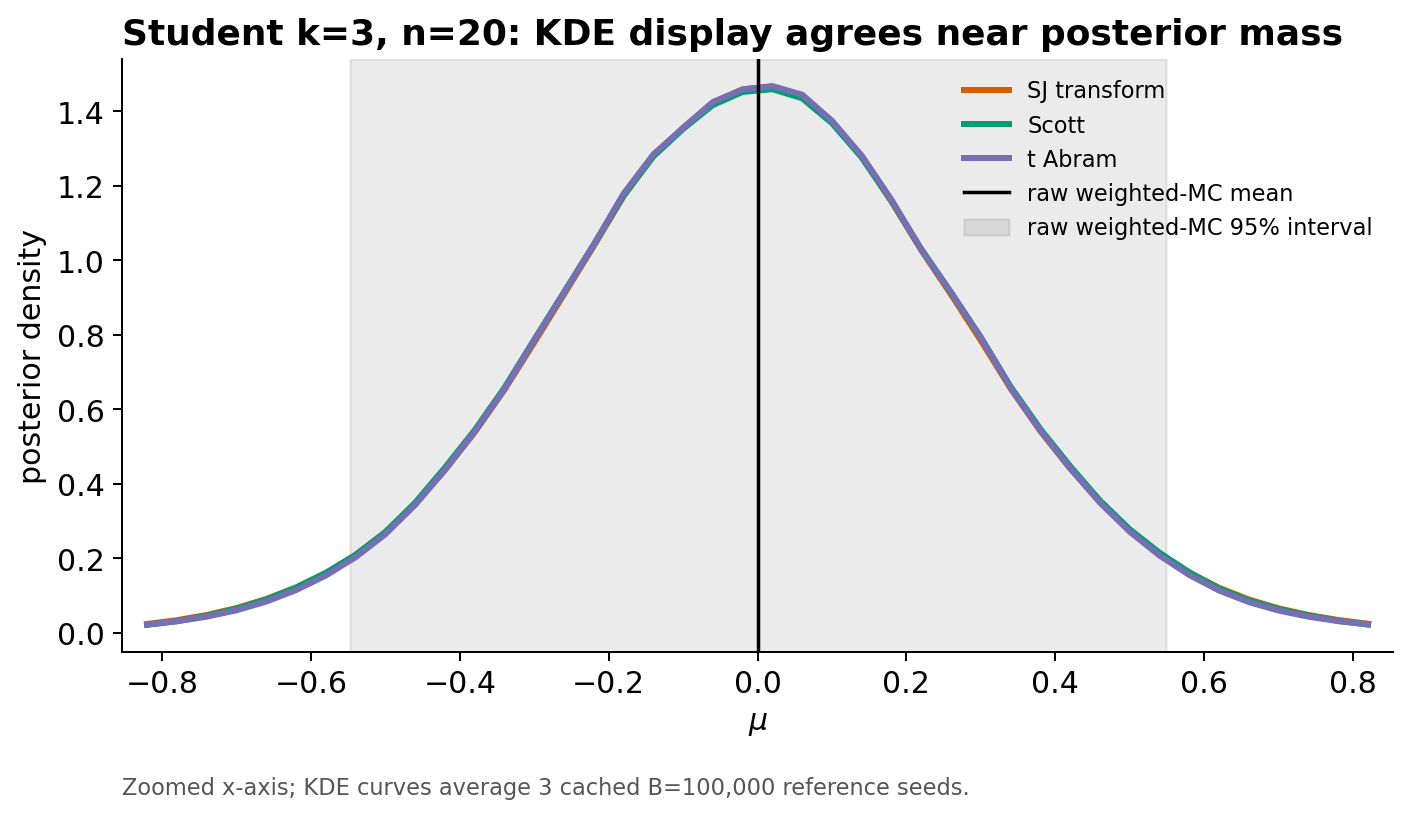
\includegraphics[width=\linewidth]{kde_density_student_k3_n20.png}
    \end{column}
    \begin{column}{0.37\textwidth}
      \claim{For Student $k=3,n=20$, smoothing is visually stable enough to support interpretation.}
      \begin{itemize}
        \item Scott is the default display backend in stable regimes.
        \item Posterior summaries still come from raw weighted-MC.
      \end{itemize}
    \end{column}
  \end{columns}
  \figsource{\texttt{results/kde\_correctness\_audit}}
\end{frame}

\begin{frame}{KDE sensitivity is part of the story}
  \begin{columns}[T,onlytextwidth]
    \begin{column}{0.58\textwidth}
      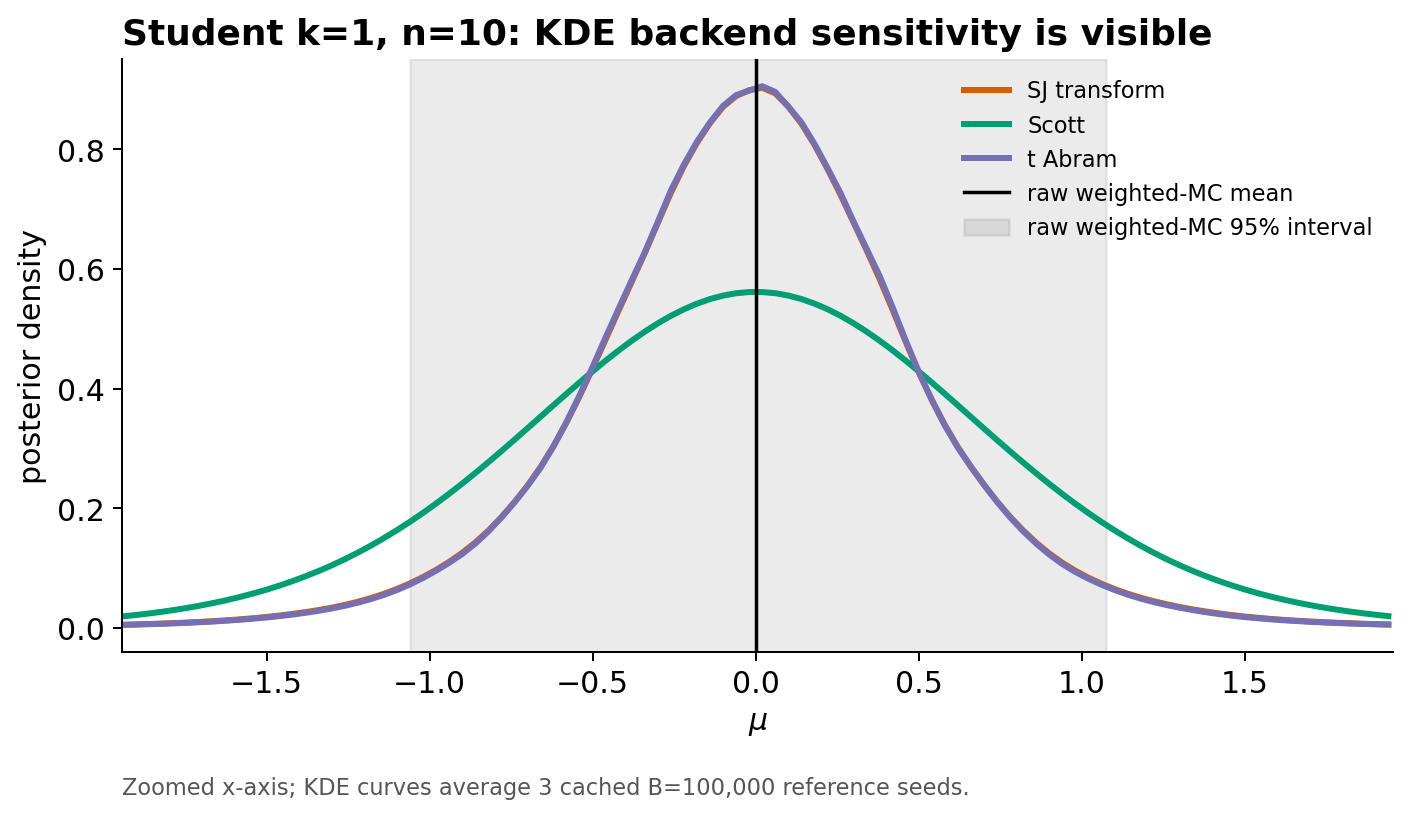
\includegraphics[width=\linewidth]{kde_density_student_k1_n10.png}
    \end{column}
    \begin{column}{0.37\textwidth}
      \claim{Student $k=1$ has no single universally reliable KDE display backend.}
      \begin{itemize}
        \item Treat as a stress-test regime.
        \item Do not let a smooth overlay decide correctness.
      \end{itemize}
    \end{column}
  \end{columns}
\end{frame}

\section{Sampler Correctness}

\begin{frame}{Correctness standard}
  \claim{A sampler passes only when the posterior summaries, invariance checks, and mixing diagnostics tell the same story.}
  \vspace{0.3cm}
  \begin{columns}[T,onlytextwidth]
    \begin{column}{0.31\textwidth}
      \begin{block}{Posterior agreement}
        Mean, SD, central and tail quantiles, central mass, Wasserstein distance versus the raw weighted-MC benchmark.
      \end{block}
    \end{column}
    \begin{column}{0.31\textwidth}
      \begin{block}{Invariant target}
        Constraint residuals, target-mismatch checks, and method-specific move identities.
      \end{block}
    \end{column}
    \begin{column}{0.31\textwidth}
      \begin{block}{Chain reliability}
        ESS/autocorrelation, split-chain drift, multiseed stability, and initialization sensitivity when cached.
      \end{block}
    \end{column}
  \end{columns}
\end{frame}

\begin{frame}{Method-specific checks}
  \claim{The diagnostics were matched to how each sampler is supposed to preserve the constrained posterior.}
  \begin{columns}[T,onlytextwidth]
    \begin{column}{0.49\textwidth}
      \begin{block}{Gibbs}
        \begin{itemize}
          \item Score-constraint residual after sweeps.
          \item Pair update preserves the pairwise $\delta$ identity.
          \item Student inverse-map branch usage is not one-sided.
          \item Seeds, splits, ESS, and latent summaries do not drift.
        \end{itemize}
      \end{block}
    \end{column}
    \begin{column}{0.49\textwidth}
      \begin{block}{RATTLE}
        \begin{itemize}
          \item Projection and tangent residuals stay near numerical zero.
          \item Reverse checks do not fail.
          \item Hamiltonian error is controlled.
          \item Gram/target correction and not-applicable cases are labeled explicitly.
        \end{itemize}
      \end{block}
    \end{column}
  \end{columns}
\end{frame}

\begin{frame}{Clean, caveat, unresolved}
  \claim{The label is a presentation decision: what can be used as evidence in the main comparison?}
  \begin{columns}[T,onlytextwidth]
    \begin{column}{0.32\textwidth}
      \begin{block}{Clean}
        Posterior agreement passes and the available invariance, geometry, and mixing diagnostics do not raise a warning.
      \end{block}
    \end{column}
    \begin{column}{0.32\textwidth}
      \begin{block}{Caveat}
        The sampler is usable as a stress-test or secondary result, but posterior agreement or mixing shows a warning.
      \end{block}
    \end{column}
    \begin{column}{0.32\textwidth}
      \begin{block}{Unresolved}
        The run is not safe as a final claim: mismatch and chain instability remain after production diagnostics.
      \end{block}
    \end{column}
  \end{columns}
  \vspace{0.25cm}
  \begin{itemize}
    \item \textbf{Clean examples:} final-production clean rows plus targeted-validation upgrades.
    \item \textbf{Main caveat:} rows where posterior or mixing warnings remain after reconciliation.
    \item \textbf{Unresolved:} Student $k=1,n=10$ for both Gibbs and RATTLE.
  \end{itemize}
\end{frame}

\begin{frame}{Reconciled sampler verdicts}
  \begin{columns}[T,onlytextwidth]
    \begin{column}{0.56\textwidth}
      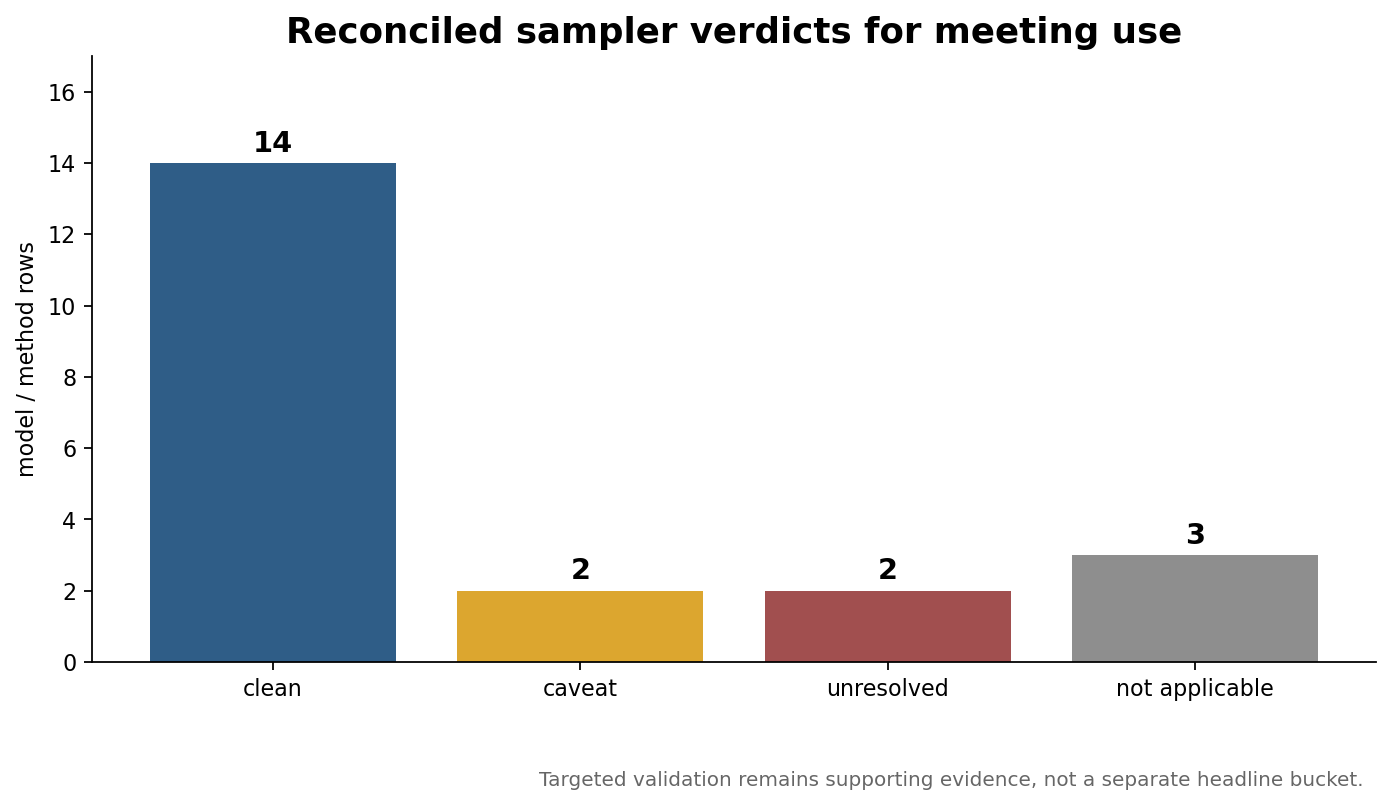
\includegraphics[width=\linewidth]{reconciled_verdict_counts.png}
    \end{column}
    \begin{column}{0.39\textwidth}
      \claim{Targeted validation upgrades 9 standalone caveats by adding multi-init and geometry evidence.}
      \begin{itemize}
        \item 14 clean production rows
        \item 9 clean with targeted support
        \item 2 remaining caveat rows
        \item 2 unresolved rows
        \item 3 not applicable rows
      \end{itemize}
    \end{column}
  \end{columns}
  \figsource{\texttt{results/meeting\_pack/reconciled\_sampler\_verdict\_table.csv}}
\end{frame}

\begin{frame}{Posterior agreement}
  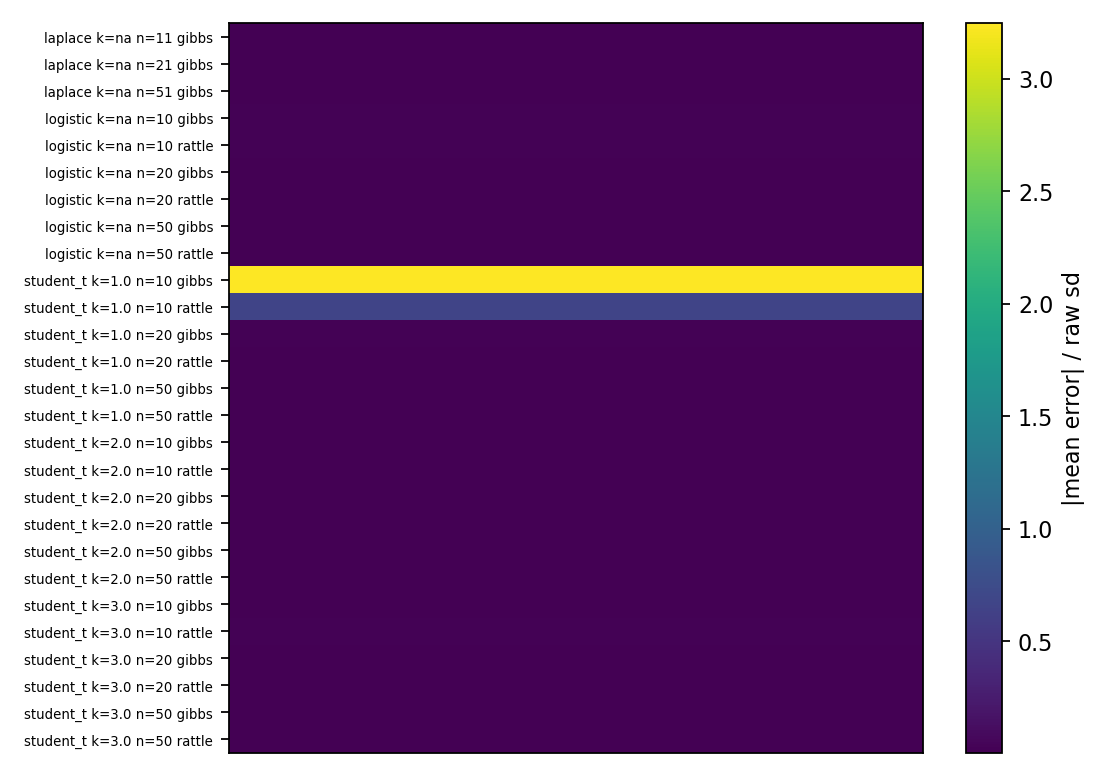
\includegraphics[height=0.64\textheight]{posterior_agreement_heatmap.png}
  \claim{Clean regimes agree with the posterior-summary benchmark; Student $k=1,n=10$ stays unresolved.}
\end{frame}

\begin{frame}{RATTLE diagnostic sanity checks}
  \begin{columns}[T,onlytextwidth]
    \begin{column}{0.49\textwidth}
      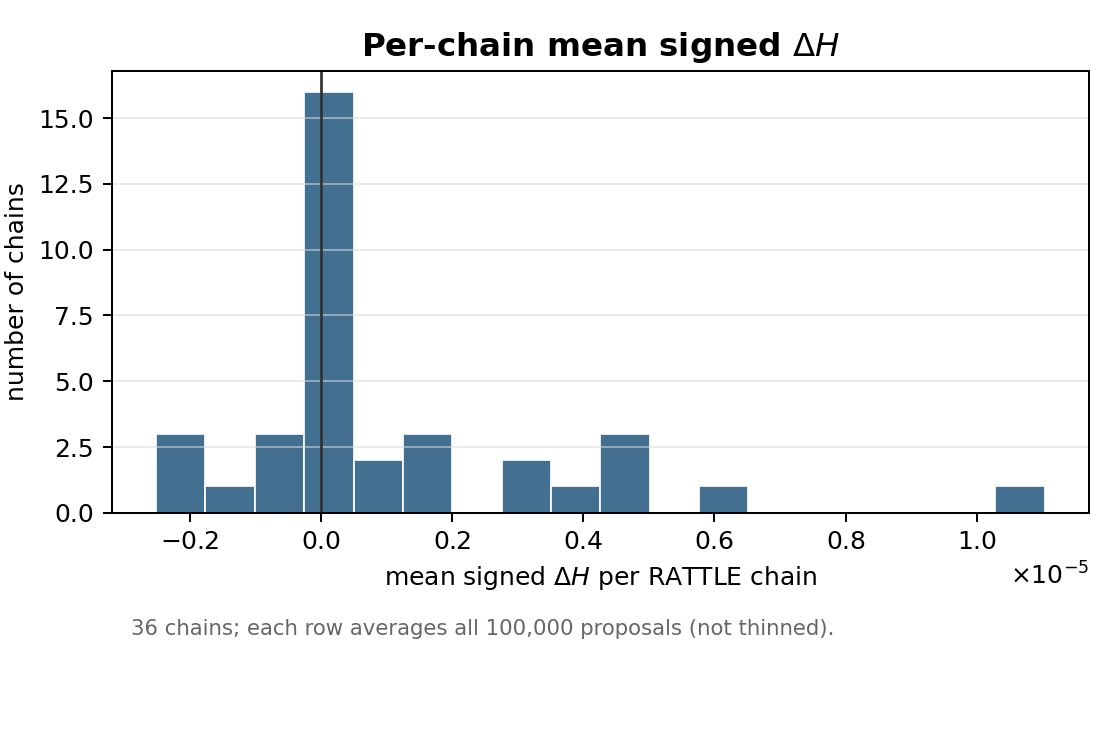
\includegraphics[width=\linewidth]{rattle_delta_H_histogram.png}
    \end{column}
    \begin{column}{0.49\textwidth}
      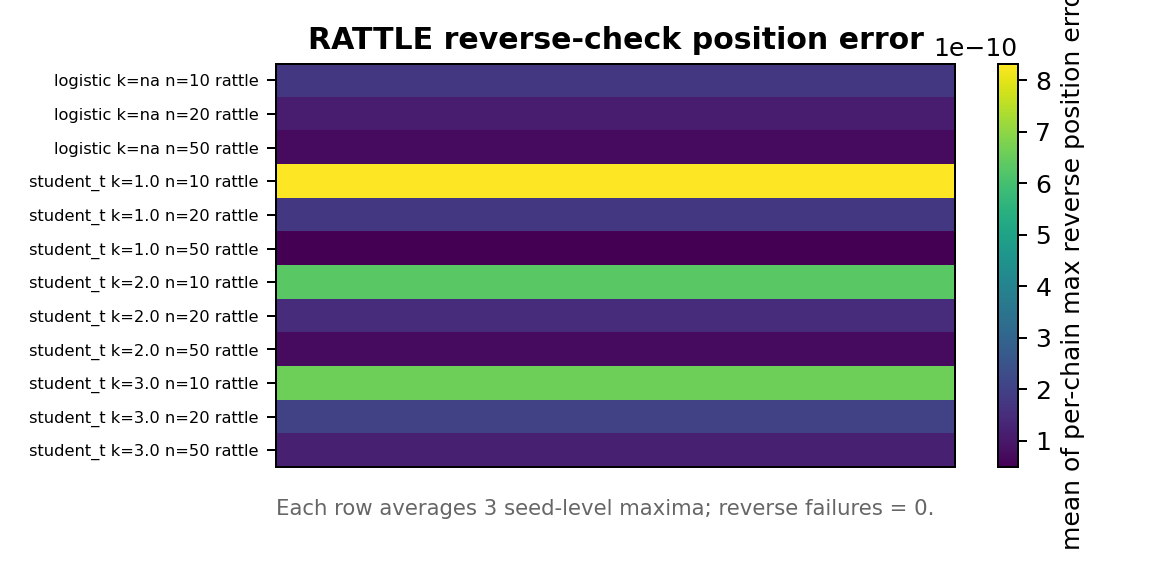
\includegraphics[width=\linewidth]{rattle_reverse_error_plot.png}
    \end{column}
  \end{columns}
  \claim{Left: per-chain mean signed $\Delta H$ over all proposals. Right: case-level mean of seed-level maximum reverse position error.}
\end{frame}

\section{Efficiency}

\begin{frame}{Efficiency question}
  \claim{The comparison is cost per reliable posterior information, not just elapsed time.}
  \begin{itemize}
    \item Raw cost: measured seconds per iteration; RATTLE is cheaper per iteration in the smooth comparable production rows.
    \item MCMC quality: ESS, autocorrelation, split drift.
    \item Final efficiency: ESS/sec for $\mu$ in rows that are safe to interpret.
  \end{itemize}
\end{frame}

\begin{frame}{Who wins in clean comparable regimes?}
  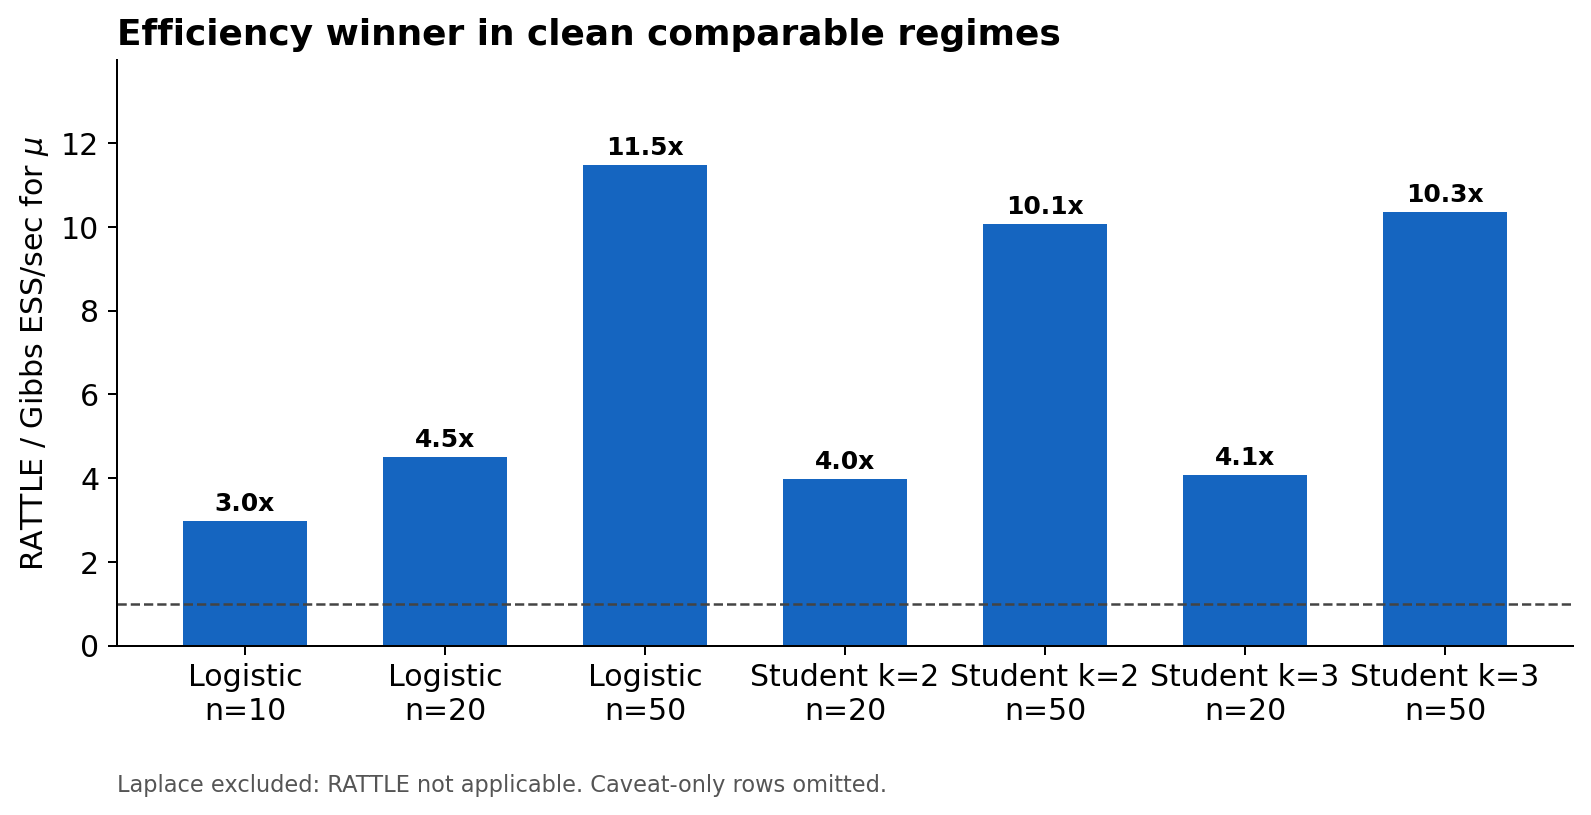
\includegraphics[height=0.64\textheight]{efficiency_ratio_main_claim.png}
  \claim{RATTLE has higher $\mu$ ESS/sec in every clean Gibbs/RATTLE production comparison.}
  \figsource{\texttt{final\_production\_v1\_efficiency\_audit\_cost\_first/method\_winners.csv}}
\end{frame}

\begin{frame}{Efficiency surface}
  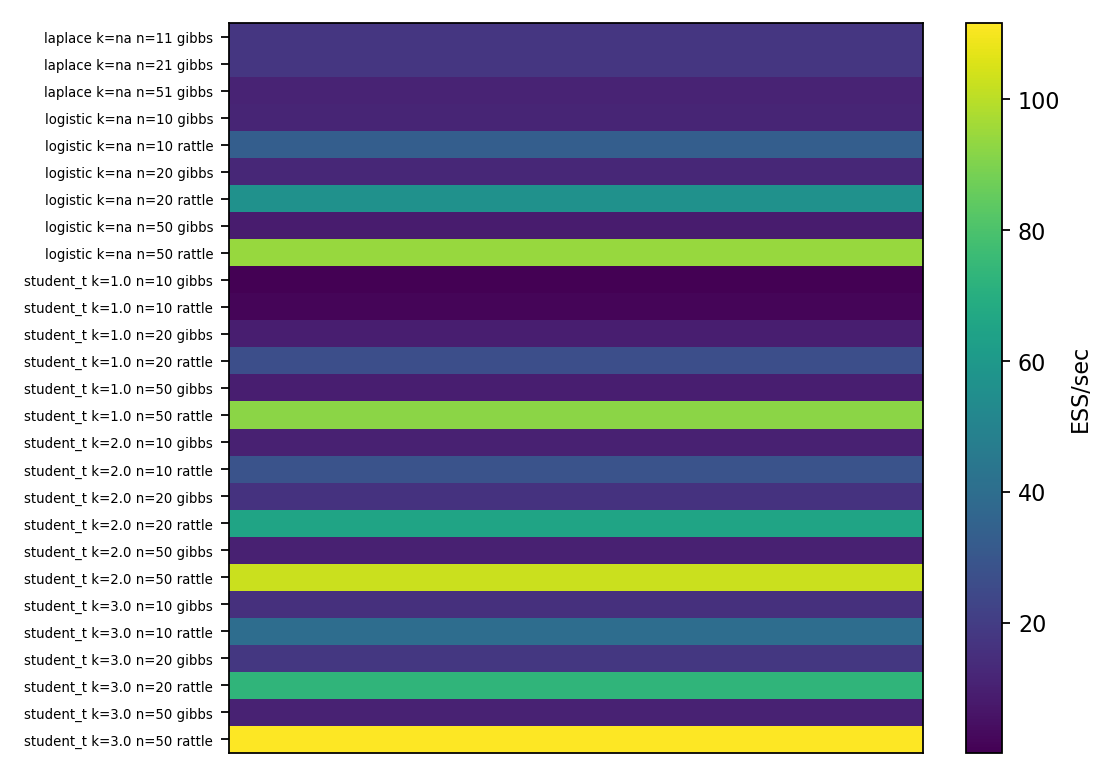
\includegraphics[height=0.63\textheight]{ess_per_sec_heatmap.png}
  \claim{The win grows with $n$ in several smooth regimes because RATTLE proposals stay cheap while Gibbs sweeps scale with latent dimension.}
\end{frame}

\section{Geometry Explanation}

\begin{frame}{Why geometry matters}
  \claim{The latent constraint creates a manifold. The winner is determined by how each sampler moves on it.}
  \begin{columns}[T,onlytextwidth]
    \begin{column}{0.49\textwidth}
      \begin{block}{Gibbs}
        Exploits algebra locally through score-preserving pair updates.
      \end{block}
    \end{column}
    \begin{column}{0.49\textwidth}
      \begin{block}{RATTLE}
        Makes geometric moves but pays projection, tangent, and Hamiltonian costs.
      \end{block}
    \end{column}
  \end{columns}
\end{frame}

\begin{frame}{Student tail geometry}
  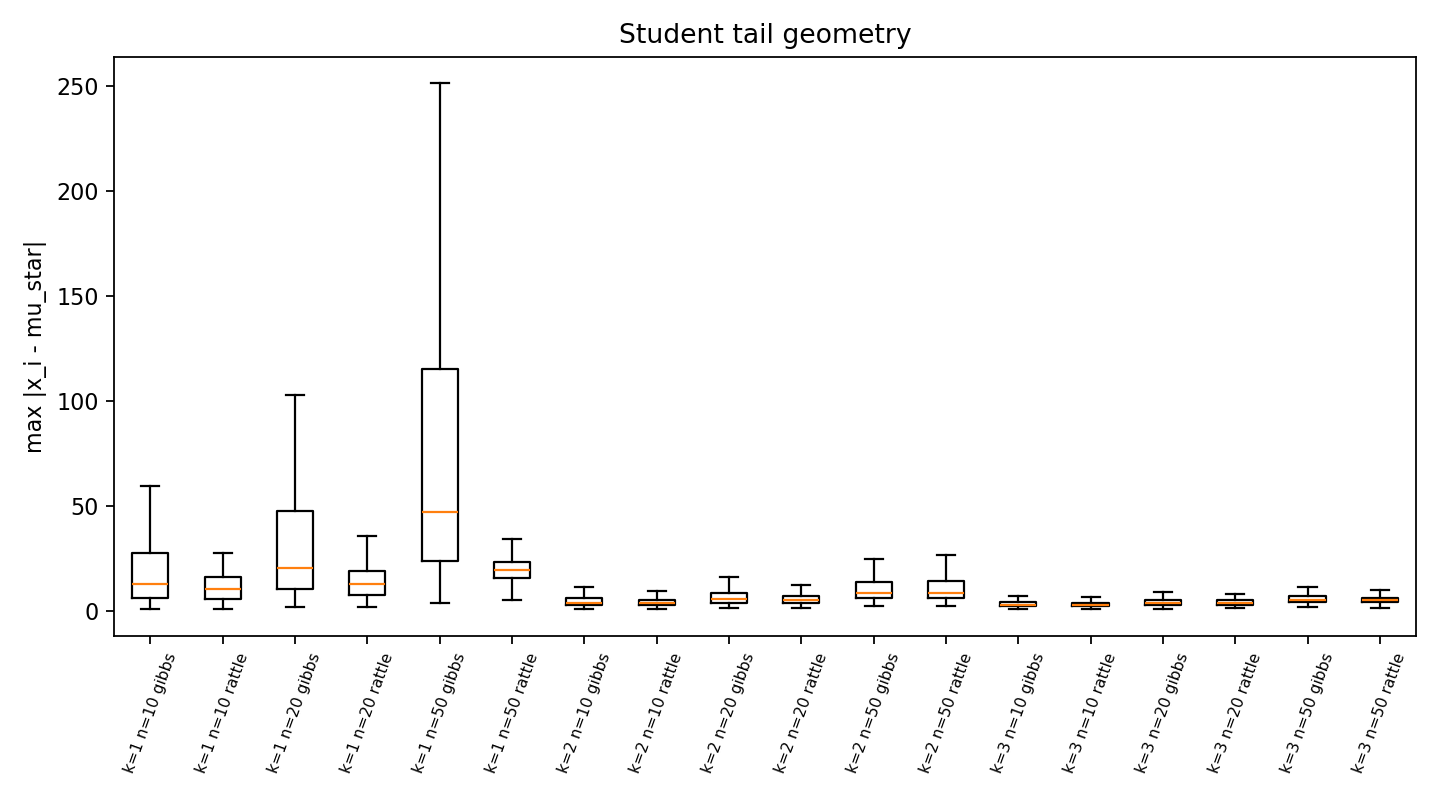
\includegraphics[height=0.62\textheight]{student_tail_geometry_histogram.png}
  \claim{Heavy tails create latent worlds with extreme observations compatible with the same $\hat{\mu}$.}
\end{frame}

\begin{frame}{Sticky latent classes}
  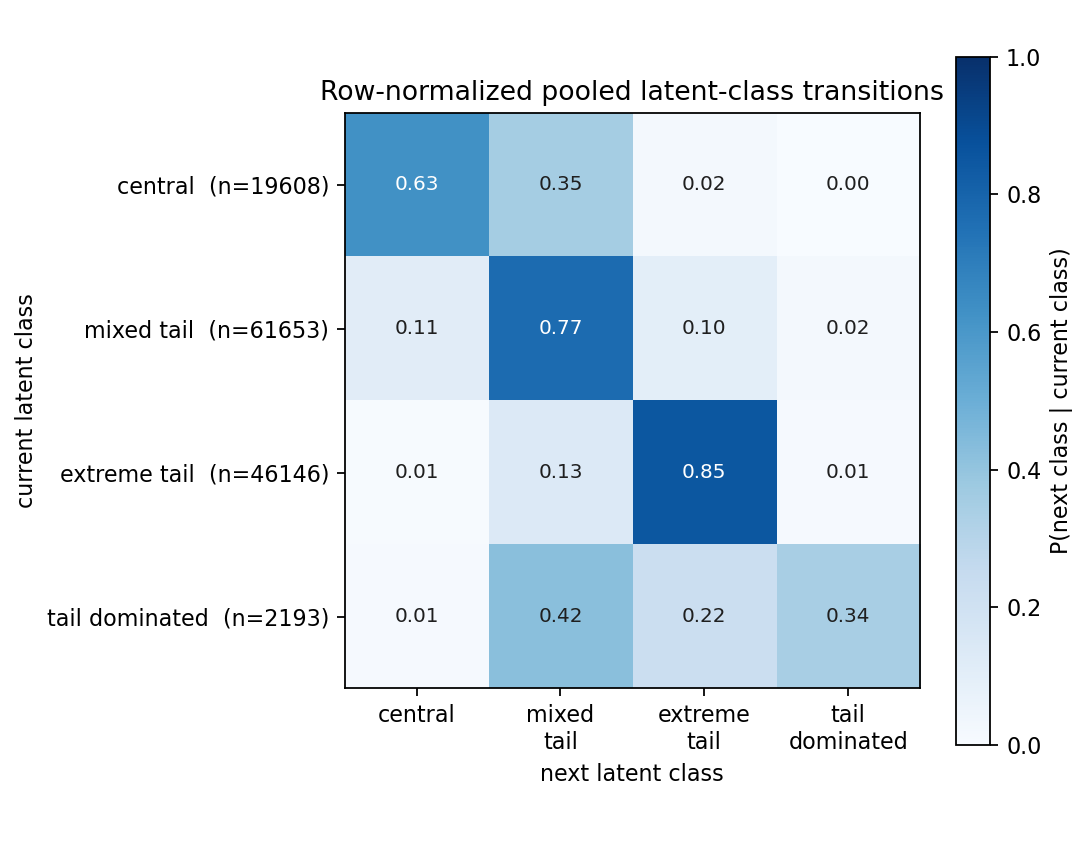
\includegraphics[height=0.62\textheight]{latent_geometry_class_transition_heatmap.png}
  \claim{The difficult cases are difficult because latent geometry classes are not explored uniformly.}
\end{frame}

\begin{frame}{Focused Cauchy follow-up}
  \claim{Student $k=1,n=50$ now gets a dedicated Gibbs geometry runset rather than another generic caveat label.}
  \begin{itemize}
    \item 15 Grace chains: 5 seeds $\times$ central, tail-heavy, and random initializations.
    \item 500k iterations, 100k burn-in, thinned full latent snapshots.
    \item New diagnostics track $z=y/(1+y^2)$, branch occupancy, extreme-tail thresholds, class switching, and geometry-conditioned $\mu$.
    \item Success criterion: explain heavy-tail geometry; do not force Student $k=1$ into a clean headline comparison.
  \end{itemize}
\end{frame}

\begin{frame}{RATTLE near tail geometry}
  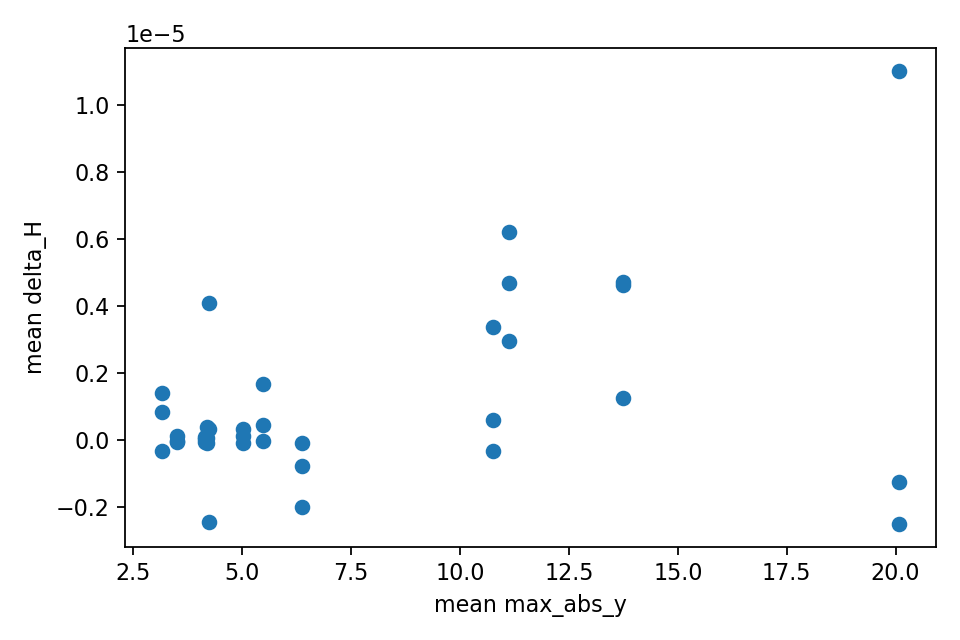
\includegraphics[height=0.62\textheight]{rattle_delta_H_vs_max_abs_y.png}
  \claim{Hamiltonian behavior degrades as latent extremes grow, which is exactly where heavy-tail regimes need care.}
\end{frame}

\section{MLE Release Payoff}

\begin{frame}{Final payoff question}
  \claim{Once the sampler is trusted, we ask what the released MLE preserves and what it leaks about hidden data.}
  \begin{columns}[T,onlytextwidth]
    \begin{column}{0.49\textwidth}
      \begin{block}{Information loss}
        Compare $p(\mu \mid x_{1:n})$ to $p(\mu \mid \hat{\mu})$ over simulated datasets.
      \end{block}
    \end{column}
    \begin{column}{0.49\textwidth}
      \begin{block}{Privacy leakage}
        Compare prior vs posterior beliefs about latent outliers compatible with $\hat{\mu}$.
      \end{block}
    \end{column}
  \end{columns}
\end{frame}

\begin{frame}{Sanity check: sufficient statistic}
  \claim{Normal known-variance gives the zero-loss reference.}
  \begin{center}
    \Large
    $p(\mu \mid \bar{x}) = p(\mu \mid x_{1:n})$
  \end{center}
  \begin{itemize}
    \item Median SD ratio: 1.000.
    \item Wasserstein and quantile differences: effectively zero.
    \item This anchors the interpretation of non-normal deviations.
  \end{itemize}
\end{frame}

\begin{frame}{Information loss in selected regimes}
  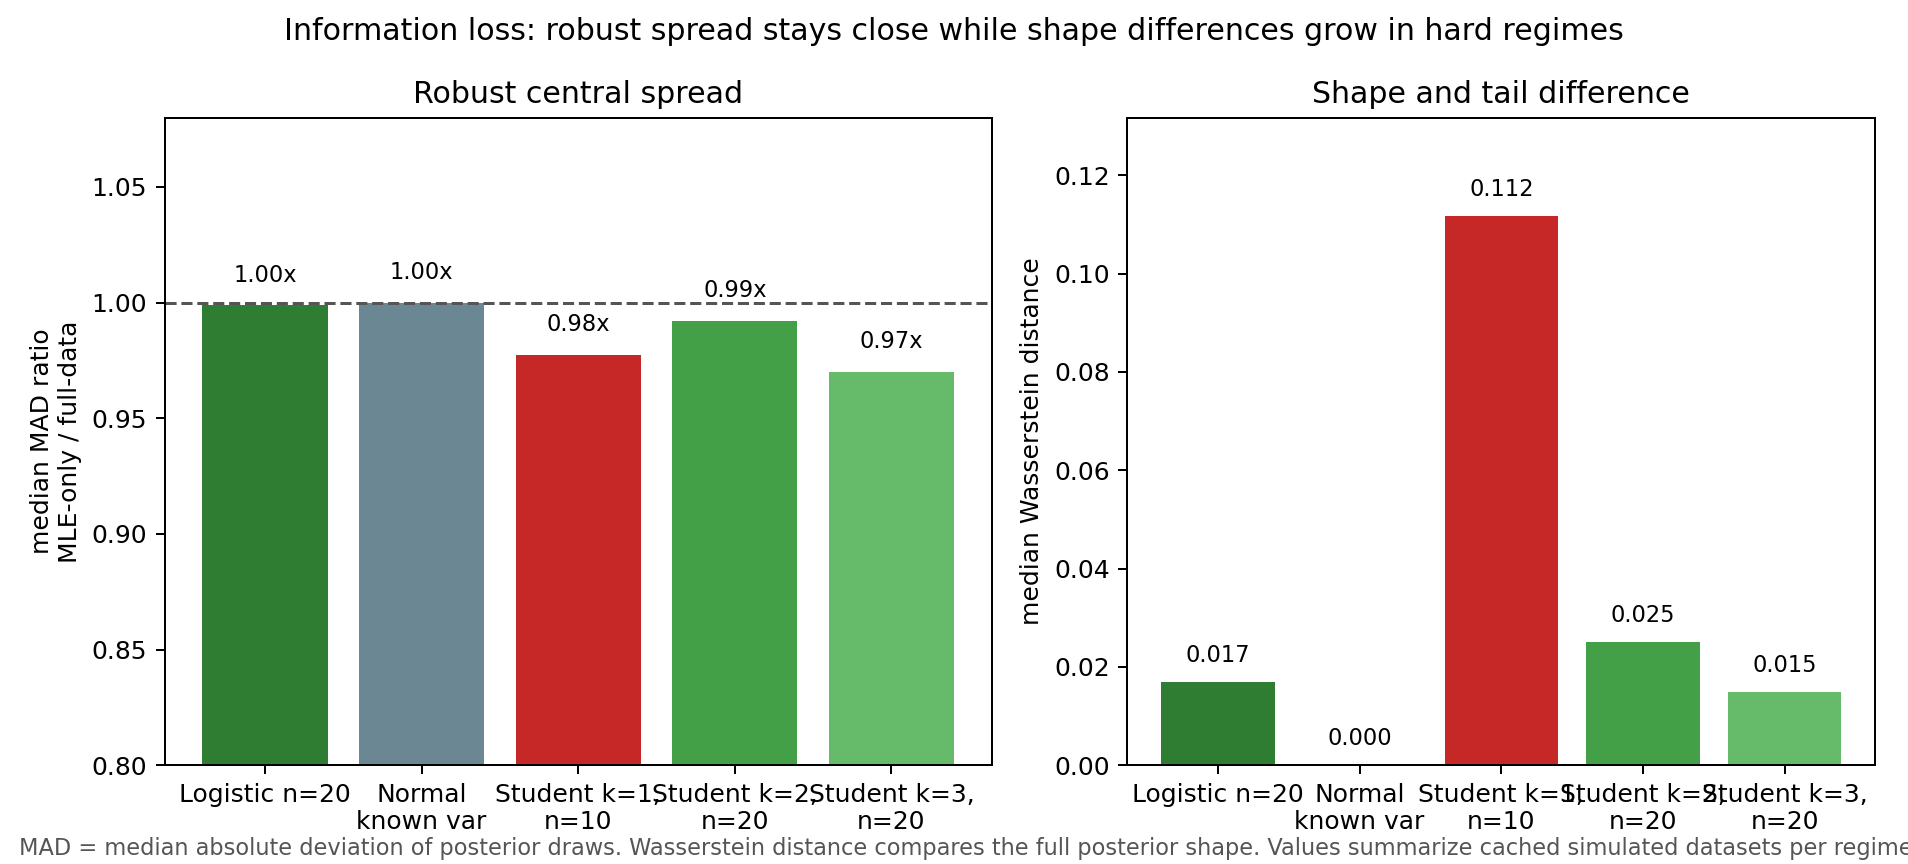
\includegraphics[height=0.65\textheight]{information_loss_selected_bars.png}
  \claim{Light/moderate tails are close; Student $k=1,n=10$ is the clear loss case.}
\end{frame}

\begin{frame}{Information loss heatmap}
  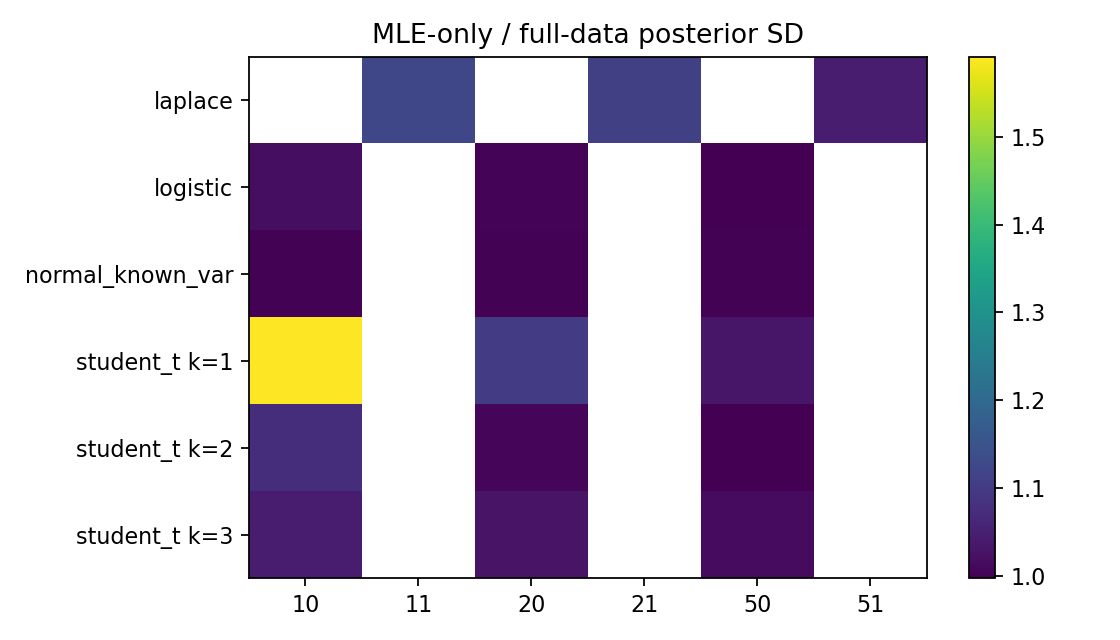
\includegraphics[height=0.63\textheight]{sd_ratio_heatmap.png}
  \claim{The broad pattern is tail- and sample-size dependent, not a universal MLE-only failure.}
  \figsource{\texttt{final\_production\_v1\_release\_information\_audit/information\_loss\_summary.csv}}
\end{frame}

\begin{frame}{Privacy-relevant leakage}
  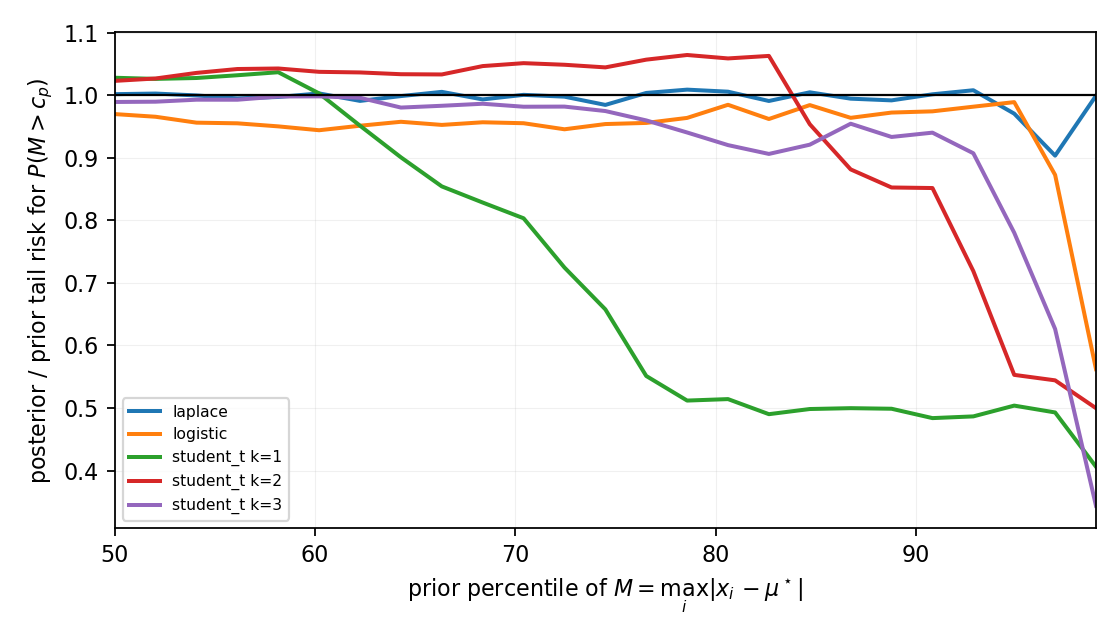
\includegraphics[height=0.63\textheight]{privacy_leakage_probability_shift.png}
  \claim{The released MLE can shift beliefs about whether compatible latent datasets contain extremes.}
\end{frame}

\begin{frame}{Same release, many compatible worlds}
  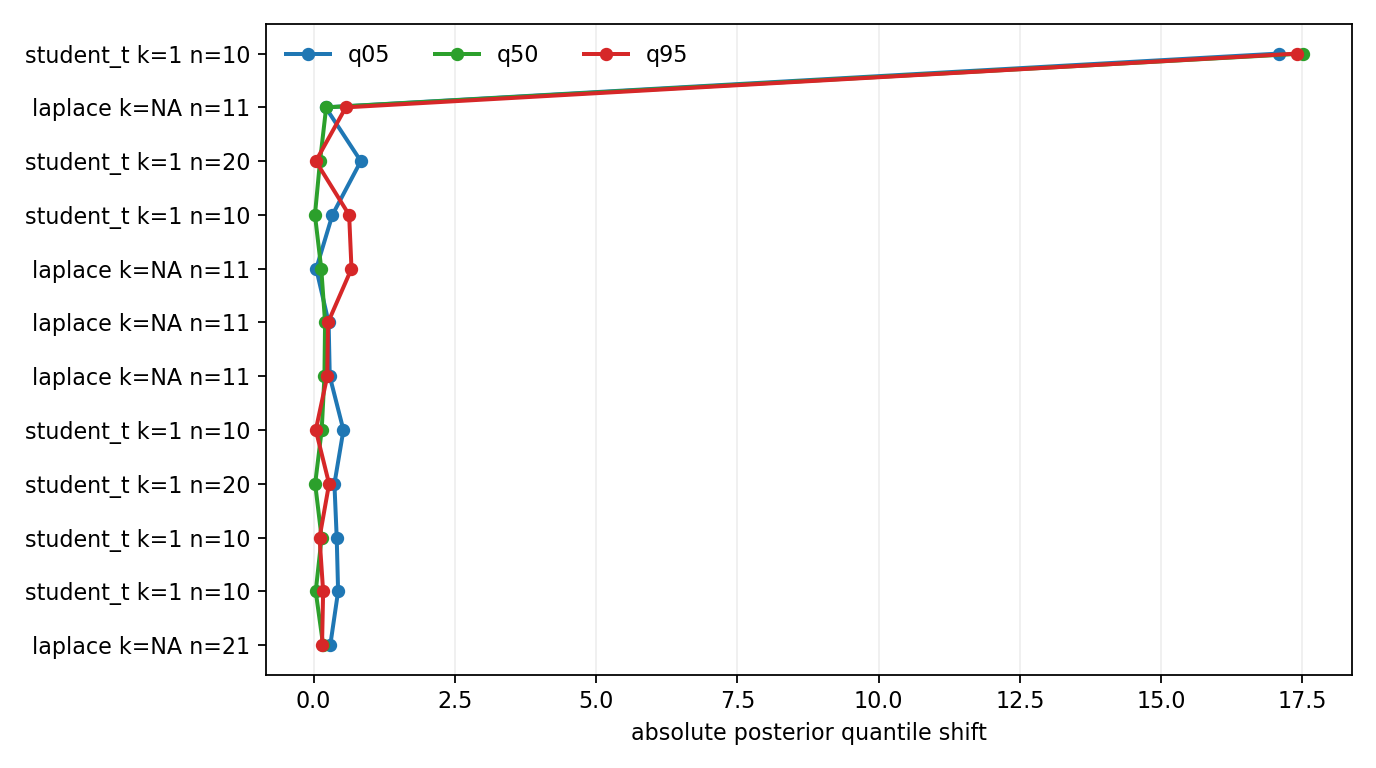
\includegraphics[height=0.63\textheight]{representative_information_loss_cases.png}
  \claim{The latent-data posterior makes visible how many different datasets can share the same released MLE.}
\end{frame}

\section{Discussion}

\begin{frame}{Dashboard walkthrough}
  \claim{Use the dashboard to drill down, but keep the meeting defaults clean.}
  \begin{itemize}
    \item Default source: \texttt{final\_production\_v1}.
    \item Posterior page: Student $k=3,n=20$ or Logistic $n=20$.
    \item KDE page: diagnostic only.
    \item Student $k=1,n=10$: caveat/unresolved.
    \item Laplace RATTLE: hidden or marked not applicable.
  \end{itemize}
\end{frame}

\begin{frame}{Caveats}
  \begin{columns}[T,onlytextwidth]
    \begin{column}{0.50\textwidth}
      \begin{block}{Do not headline}
        \begin{itemize}
          \item Student $k=1,n=10$
          \item Student $k=1$ broader heavy-tail claims
          \item Caveat-only small-$n$ rows
        \end{itemize}
      \end{block}
    \end{column}
    \begin{column}{0.46\textwidth}
      \begin{block}{Keep explicit}
        \begin{itemize}
          \item Laplace RATTLE is not applicable
          \item KDE is diagnostic smoothing
          \item Privacy result is belief-shift leakage
        \end{itemize}
      \end{block}
    \end{column}
  \end{columns}
\end{frame}

\begin{frame}{Takeaway}
  \claim{The pipeline now supports a coherent story: validate the sampler, compare efficiency, explain behavior geometrically, then use the trusted sampler to quantify information loss and privacy-relevant leakage.}
  \begin{enumerate}
    \item Clean regimes support Gibbs/RATTLE comparison.
    \item RATTLE is more efficient in smooth comparable regimes.
    \item Heavy tails explain the remaining caveats.
    \item MLE-only release is benign in some regimes and lossy/leaky in others.
  \end{enumerate}
\end{frame}

\end{document}
